\documentclass[10pt]{report}
\usepackage[utf8]{inputenc}
\usepackage[italian]{babel}
\usepackage{multicol}
\usepackage[bookmarks]{hyperref}
\usepackage[a4paper, total={18cm, 25cm}]{geometry}
\usepackage{graphicx}
\usepackage{xcolor}
\usepackage{textcomp}
\graphicspath{ {./img/} }
\usepackage{listings}
\usepackage{makecell}
\lstdefinestyle{customasm}{
  belowcaptionskip=1\baselineskip,
  frame=line,
  xleftmargin=\parindent,
  language=[x86masm]Assembler,
  basicstyle=\ttfamily,
  commentstyle=\itshape\color{purple!40!black},
}
\lstset{escapechar=@,style=customasm}
\lstnewenvironment{C}
  {\lstset{language=C++,frame=none}}
  {}
\begin{document}
\title{Artificial Intelligence Fundamentals}
\author{Federico Matteoni}
\date{A.A. 2021/22}
\renewcommand*\contentsname{Index}

\maketitle
\begin{multicols}{2}
\tableofcontents
\end{multicols}
\pagebreak
\section{Introduction}
Prof.s: Maria Simi, Vincenzo Lomonaco\\
AI is taking over the world. Formalizing common sense is a lot more difficult. We can formalize knowledge in very specific and small domains. But is deep learning the final solution to AI? "It will transform many industries, but it's not magic. Almost all of AI's recent progress is based on one type of AI, in which some input is used to quickly generate simple response." (\textit{Andrew Ng})\\
\textit{This} AI can do supervised learning, but requires huge amount of data (tens of thousands of pictures to build a photo tagger, for example). The rule of thumb of Ng is: if a person can do a mental task with less than one second of thought, we can automate it using AI either now or in the near future.\\
The challenges are:
\begin{list}{}{}
	\item Software is not a problem, the community is open and the software can be replicated the software can be replicated
	\item Data is exceedingly difficult to get access to. Data is the defensible barrier for many businesses
	\item Talent, because downloading and applying open-source software to your data won't work. AI needs to be customized to context and data, that's why there's a war for the scarce AI talent that can do this work.
	\item Computational resources are also very important.
\end{list}
\paragraph{Deep Learning} Is only one approach inside the much wider field of ML and ML is only one approach in the wider field of AI. Book: \textit{Thinking Fast and Slow}, Kahneman. Two systems: system 1 does perceptual tasks, simple computations, system 2 instead does complex computation, recalling from memory\ldots this is a distinction in our brains.
\paragraph{Machine Learning} Is AI all about machine learning? Possible arguments against ML are:
\begin{list}{}{}
	\item Explanation and accountability: ML systems are not (yet?) able to justify in human terms their results. For some applications this is essential: knowledge must be meaningful to humans to be able to generate explanations? Some regulations requires the right to an explanation in decision-making, and seek to prevent discrimination based on race, opinions, sex\ldots (see GDPR)
	\item ML systems learn what's in the data, \textbf{without understanding what's true or false, real or imaginary, fair or unfair}. It is possible to develop unfair, bad models. People are generally more critical about information.
\end{list}
Building AI systems is a goal far from being solved, still quite challenging. Complex AI systems requires the combination of several techniques and approaches, not only ML.
\paragraph{AI Fundamentals} Is mostly about reasoning and \textit{slow thinking}. Different approaches, "good old-fashioned artificial intelligence" or "symbolic AI": teaching about the foundations of the discipline, now 60 years old.
\paragraph{Symbolic AI} High-level human readable representations of problems, the general paradigm of searching for a solution, knowledge representation and reasoning, planning. Dominant paradigm from the mid 1950s until late 1980s.\\
Central to the building of AI systems is the physical symbol systems hypothesis (PSSH), formulated by Newell and Simon (\textit{Computer Science as Empirical Inquiry: Symbols and Search})\\
The approach is based on the assumption that many aspects of intelligence can be achieved by the manipulation of symbols (the PSSH): \textit{a physical symbol system has the necessary and sufficient means for general intelligent action}.\\
Human thinking is a king of symbol manipulation system (so a symbol system is \textbf{necessary} for intelligence), and machine can be intelligent (a symbol system is \textbf{sufficient} for intelligence). This cannot be prove, we can only collect empirical evidence: observation and experiments on human behavior in tasks requiring intelligence, and solving tasks of increasing complexity.
\paragraph{Strong and Weak AI} The Chinese room argument, by John Searle, introduced the following distinction: strong ai relies on the \textit{strong} assumption that human intelligence can be reproduced in all its aspects (general AI), including adaptivity, learning, consciousness\ldots, while weak AI is the simulation of human-like behavior, without effetctive thinking or understanding, no claim that it works like the human mind. Dominant approach today, fragmented AI.\\
One strong argument against strong AI is the lack of needs by the systems: biological need, safety, relationships, self esteem, self-actualization (Maslow's hierarchy of needs).\\
\textit{What stands in the way of all-powerful AI is not a lack of smarts: it's that computers can't have needs, cravings or desires.}\\\\
\textbf{AI is the enterprise of building intelligent computational agents}
\paragraph{Agents} An agent is something that acts in an environment. We are interested in what an agetn does, that is how it acts. We judge and agent by its action. An agent acts intelligently when: what it does is appropriate given the circumnstances and its goals, it is flexible to changing envoronments and changing goals, learns from experience, makes appropriate choices given its perceptual and computational limitations.\\
\textbf{Computational agent} is an agent whose decsiions about its actions can be explained in terms of computation and implkemented on a physical device.
\begin{list}{}{}
	\item \textbf{Scientific Goal}: undestrand the principles that make intelligent behavior possibile in natural or artificial systems
	\item \textbf{Engineering Goal}: design and synthesis of userful, intelligente artifacts, agents that are useful in many applications
\end{list}
%TODO lista slide 5
\paragraph{Artificial Intelligence} Artificial intelligent is not the opposit of real intelligence. Intelligence cannot be \textit{fake}: in an artificial agent behaves intelligently, it is intelligent. It is only the external behavior that defines intelligence, according to the \textbf{Turing Test} (weak AI). So \textbf{artificial intelligence is real intelligence created artificially}.\\
More updated test: Winograd schemas.\\
\textbf{Human intelligence}: biology (surviving various habitats), culture (language, tools, concepts, wisdom passed from parents and teachers to children) and life-long learning experience (learning throughout life). Another form is social intelligence, exhibited by communities and organizations.\\\\
So agents are situated in environments, inputs are abilities, goals, prior knowledge, stimuli and past experiences, and outputs actions which affect the environment.
\begin{center}
	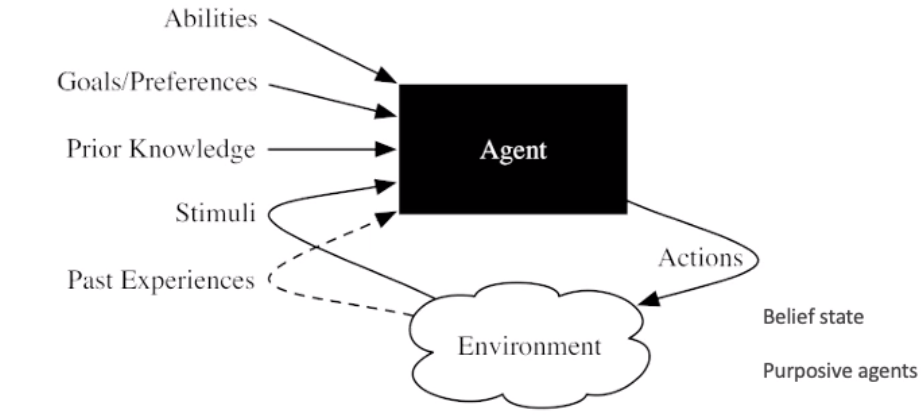
\includegraphics[scale=0.5]{1.png}
\end{center}
\paragraph{Design process}
\begin{list}{}{}
	\item design time computation, that goes into the design
	\item offline computation, that the agent can do before acting in the world (ex: specializing the model)
	\item online computation, done by the agent that is acting
\end{list}
Designing an intelligent agent that can adapt to complex environments and changing goals is a major challenge. Two strategies: simplify environments and build strong reasoning systems for these simple environments, or build simple agents for natural/complex environments simplifying the task.\\
\textbf{Steps} in the design process:
\begin{list}{}{}
	\item define the task in natural language, what need to be computed
	\item define what is a solution and its quality: optimal, satisfying, aproximately optimal, probable\ldots
	\item formal representation for the task, choosing how to represent knowledge for the task, including representations suitable for learning.
	\item compute an output
	\item interpret output as solution
\end{list}
\begin{center}
	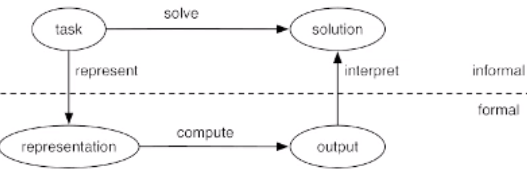
\includegraphics[scale=0.5]{2.png}
\end{center}
\paragraph{Levels of abstraction} A model of the world is a syumbolic rtepresentation of the beliefs of the agents. In is necessarily an abstraction: more abstract representations are simpler and human-readable but they may not be effective enough. Low level descriptions are more detailed and accurate but more complex too. Multiple level of abstractions are possibile (hierchical design). Two levels always present in the design: knowledge level (what the agent knows and its goals, not in terms of how we represent) and the symbol level (internal representation and reasoning system). \textbf{Modularity} extent to which a system/task can be decomposed \begin{list}{}{}
	\item flat: not modular
	\item modular: interacting modules that can be understood on their own
	\item hierarchical: modules are decomposed into simpler modules
\end{list}
\textbf{Planning horizon} how far ahead in time the agent plans \begin{list}{}{}
	\item non planning agent
	\item finite horizon planner: looks for a fixed amount of stages, greedy if only one step ahead
	\item indefinite horizon planner: finite but not predetermined number of stages
	\item infinite horizon planner: keeps planning forever (ex: stabilization module of a legged robot)
\end{list}
\textbf{Representation} concerns how the state of the world is described \begin{list}{}{}
	\item Atomic states
	\item feature-based representation: set of propositions that are true or false (PROP, CSP, most ML)
	\item individuals and relations, or relational representation
\end{list}
\textbf{Computational limits} that determines whether an agent has \begin{list}{}{}
	\item perfect rationality, reasons about the best actions without constraints
	\item bounded rationality, decides on the best action that it can find given its limits
\end{list}
An anytime algorithm is an algorithm where the solution improves with time.\\
\textbf{Learning dimensions} determines whether \begin{list}{}{}
	\item knowledge is given in advance, or
	\item knowledge is learned (from data or past experience)
\end{list}
Learning typically means finding the best model th %TODO
\textbf{Uncertainty}, which can be \begin{list}{}{}
	\item in sensing (fully/partially observable states)
	\item about the effects of the actions (deterministic/stochastic)
\end{list}
\textbf{Preference} dimension which considers thetehr the agent has
\begin{list}{}{}
	\item goal (achievemtn goal a proposition true in a final state, or mainentance goal, proposition true in all psobbile states)
	\item complex preferences, involving trade-offs among the desiderability of various\ldots %TODO
\end{list}
\textbf{Number of agents}\begin{list}{}{}
	\item single agent reasoning
	\item multi agent resoning
\end{list}
\textbf{Interaction} considers wheter the agent does:
\begin{list}{}{}
	\item offline reasoning or
	\item online reasoning
\end{list}
\paragraph{Agent Architectures} Agent interacts with an environment, receives informations with sensors and acts in the world with actuators. Robot: physical body. Program: software agent, digital environment.\\
Agent is made of body and controller, which receives percepts from the body and sends command to the body. A body includes sensors that converts stimuli into percepts and actautors that convert commands into actions.
\begin{center}
	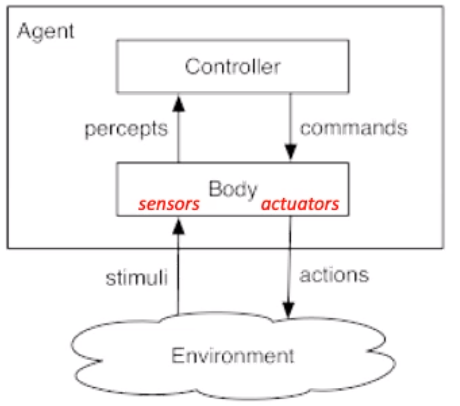
\includegraphics[scale=0.5]{3.png}
\end{center}
Bot sensors and %TODO
Agents act in time. $T$ is a set of time points, with start at 0, totally ordered, discrete and each $t$ has a next time $t+1$.\\
Percept trace/stream: function of time into percepts (past, present, future)\\
Command trace: a function of time into commands (past, present, future)\\
History at time $t$: percepts up to $t$ and commands up to $t-1$
\paragraph{Causal Trasduction} Function from history to commands. Transduction comes from \textit{finite state transducers}, where both new states and commands are emitted. "Causal" because only previous and current percepts and previous commands can be considered. A controller ideally implements a causal transduction.\\
But complete history is usually unavailable, only the memory of it. The belief state of an agent at time $t$ is all the information that the agent remembers from the previous times. The behavior of an agent can be described by two functions:
\begin{list}{}{}
	\item \textbf{Belief State function} $\textsl{remember}:S\times P\rightarrow S$ with $S$ being the set of belief states and $P$ the set of percepts
	\item \textbf{Command function} $\textsl{command}:S\times P \rightarrow C$ with $C$ being the set of commands.
\end{list}
The controller implements both, an approximation of the causal transduction.
\paragraph{Problem Solving as search} The dominant approach to AI is formulating a task as a search in a state space. The paradigm is as follows:
\begin{list}{}{}
	\item Define a goal (a set of states, a boolean test function\ldots)
	\item Formulate the task as a search problem: define a representation for states and define legal actions and transition functions
	\item Find a solution (a sequence of actions) by means of a search process
	\item Execute the plan
\end{list}
This is a basic technique in AI: search happens inside the agent, it's the planning stage before acting. It's different from searching the world, when an agent may have to act in the world and interleave an action with planning.\\
Search is a general paradigm, underlying much of the artificial intelligence field. An agent is usually given only a description of what it should achieve, not an algorithm to solve it. The only possibility is to search for a solution. Searching can be computationally very hard (NP-Complete).\\
Humans are able to solve specific instances by using their knowledge about the problem. This extra knowledge is called \textbf{heuristic knowledge}.
\paragraph{Assumptions in classic problem solving} Problem solving agents are goal driven agents, that work under simplified assumptions made in the design process.
\begin{list}{}{}
	\item States are treated as black boxes: we only need to know the heuristic value and whether they are a goal by applying the boolean goal function. The internal structure doesn't matter from the point of view of search algorithms. \textbf{Atomic representations}.
	\item The agent has \textbf{perfect knowledge} of the state (full accessibility), no uncertainty in sensors.
	\item Actions are \textbf{deterministic}, so that the agent know the consequences of its actions.
\end{list}
The state space is generated incrementally: can be infinite, so may not fit in memory.
\paragraph{Problem formulation} A problem is defined formally by five components:
\begin{list}{}{}
	\item \textbf{Initial state}
	\item \textbf{Possible actions} in state $s$, $\textsl{Actions}(s)$
	\item \textbf{Transition model}: a function $\textsl{Result}: \textsl{State}\times\textsl{Action}\rightarrow \textsl{State}$\\
	$\textsl{Result}(s,a) = s'$, a \textbf{successor state}
	\item \textbf{Goal states} are defined by a boolean function\\
	$\textsl{Goal-Test}(s) \rightarrow\{\textsl{true}, \textsl{false}\}$
	\item $\textsl{Path-cost}$ function, that assigns a numeric cost to each path. The sum of the cost of the actions on the path $c(s, a, s')$
\end{list}
\paragraph{Graphs for searching} A (directed) graph consists of a set $N$ of nodes and a set $A$ of arcs, which are ordered pairs of nodes. Node $n_2$ is a neighbor/successor of $n_1$ if $\exists\:(n_1, n_2)\in A$, and a path is a sequence of nodes $(n_0,\ldots,n_k)$ such that $(n_{i-1}, n_i)\in A$ with length $k$.\\The cost of the path is the sum of the costs of its arcs $\textsl{cost}((n_0,\ldots,n_k)) = \sum_{i=1}^k \textsl{cost}((n_{i-1}, n_i))$.\\
A \textbf{solution} is a path from a start node to a goal node and an \textbf{optimal solution} is one with minimum cost.
\paragraph{Search algorithms} A problem is given as input to a search algorithm. A solution to a problem is a path (actions sequence) that leads from the initial state to a goal state.\\
\textbf{Solution quality} is measured by the path cost function and an optimal solution has the lowest path cost among all solutions. Different strategies (algorithms) for searching the state space may be characterized by:
\begin{list}{}{}
	\item Their time and space complexity, completeness, optimality\ldots
	\item Uninformed search methods vs informed/heuristic search methods, which use an heuristic evaluation function of the nodes
	\item Direction of search (forward or backwards)
	\item Global vs local search methods
\end{list}
\subparagraph{Generic search algorithm}
\begin{verbatim}
	input:
		a graph
		a set of nodes
		boolean function goal(n) that tests if n is a goal node
	
	frontier := {s | s is a start node}
	while frontier is not empty:
		select and remove path (n0, ..., nk) from frontier
		if goal(nk):
			return (n0, ..., nk)
		for each neighbor n of nk
			add (n0, ..., nk, n) to frontier
	end while
	return fail
\end{verbatim}
\subparagraph{Other algorithms} With $b$ max number of successors, $d$ depth of solution and $m$ max distance of solution. \begin{list}{}{}
	\item \textbf{Breadth and Depth search} Respectively:
		\begin{center}
			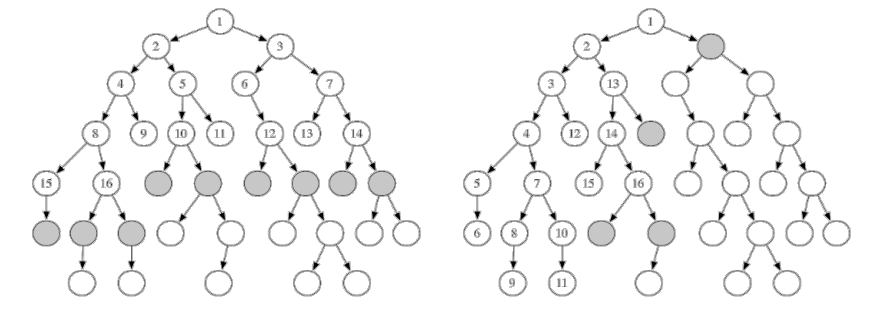
\includegraphics[scale=0.75]{4.png}
		\end{center}
		\textbf{Breadth search}: complete, optimal, time $O(b^d)$, space $O(b^d)$\\
		\textbf{Depth search}: not complete, time $O(b^m)$, space $O(bm)$
	\item \textbf{Depth bounded search}: supposes to know the distance of the solution, performs depth-first up to a limit without giving up completeness
	\item \textbf{Iterative deepening}: tries depth limit 1, then 2, then 3 and so on, freeing memory from one iteration to the next.
	\item \textbf{Uniform cost search}: at each stage, selects a path on the frontier with lowest cost.\\
	The frontier is priority queue ordered by path cost, so the first path to goal is the least-cost path. When arc costs are equal is equivalent to breadth-first search.\\
	This strategy is complete, provided that the branching factor is finite and there is some $\epsilon > 0$ such that all the costs are $> \epsilon$. It's also optimal, since it guarantees that the paths with lower costs are found first.
\end{list}
\subparagraph{Heuristic search} The idea is to not ignoring the goal when selecting the paths. Often there's extra knowledge that can be used to guide the search: \textbf{heuristics}, provided by an heuristic function $h:N\rightarrow R \Rightarrow h(n)$ is the estimate of the cost of the shortest path from node $n$ to the goal node.\\
$h$ needs to be efficiently to compute. An \textbf{admissible heuristic} $h^*(n)$ is a non-negative heuristic function that \textbf{under-estimates} the minimum cost of a path from a node $n$ to a goal: $\forall\:n\:\:\:h(n) \leq h^*(n)$\\\\
\textbf{Best first search} selects the most promising node on the frontier according to the heuristic function.
\subparagraph{$A^*$ search} With an heuristic function in the form $f(n) = g(n) + h(n)$ with:
\begin{list}{}{}
	\item $g(n)$ being the cost of path leading to $n$ (so the previous path up until $n$, $\textsl{cost}(n)$)
	\item $h(n)$ is an admissible heuristic (so, $h(n) \geq 0$)
\end{list}
Then $f(n)$ estimates the total path cost of going from a start node to a goal via $n$. The special cases are $h = 0$ (lowest cost search) and $g = 0$ (greedy best first).\\
Properties of $A^*$:\begin{list}{}{}
	\item Complete
	\item Always finds an optimal solution, if the branching factor is finite and arc costs are bounded above 0 (which means that $\exists\:\epsilon > 0\:|$ arc costs are $> \epsilon$)
	\item Optimiziations are possibile when searching graphs
	\item The operate some sort of graph pruning:
	\begin{list}{}{}
		\item \textbf{Cycle pruning}: doesn't add nodes to the frontier with states already encountered along the path (easy)
		\item \textbf{Multiple-path pruning}: maintains an explored set of nodes that are at the end of paths that have been expanded. When an $n$ is selected, if its state is already in the explored set, it's discarded.
	\end{list}
	\item Memory requirement is exponential ($O(b^d)$). Can be mitigated in some ways:
	\begin{list}{}{}
		\item $IDA^*$: performs repeated depth-bounded searches with value of $f(n)$ used as bound
		\item Recursive best-first, similar to branch \& bound
		\item $SMA^*$ (simplified memory-bounded $A^*$)
		\item Beam search, keeps in frontier only the best $k$ paths, with $k$ being the beam width (gives up optimality)
	\end{list}
\end{list}
\subparagraph{Consistent heuristics} An heuristic that statisfies the monotone restriction guarantees consistency $h(n) \leq \textsl{cost}(n, n') + h(n')$\\
Consistency $\Rightarrow$ admissibility. With the monotone restriction, the $f$-values of the paths selected from the frontier are monotonically non-decreasing.
\paragraph{Features} Often better to describe states in terms of features: \textbf{factored representation}, more natural and efficient than explicitly enumerating states. Often, features are not independent and there are constraints that specify legal combinations of assignments. We can exploits these constraints to solve tasks.\\
Constraint satisfaction is about generating assignments that satisfy a set of hard constraints and how to optimize a collection of soft constraints (preferences).
\paragraph{CSP} \textbf{Constraint Satisfaction Problem}, formal definition.
A Constraint Satisfaction Problem $CSP = \langle X, D, C\rangle$ consists of three components: \begin{list}{}{}
	\item A finite set of \textbf{variables}, $X = \{x_1, \ldots, x_n\}$
	\item A \textbf{finite domain} for each variable, $D = \{D_1, \ldots, D_n\}$ with each $D_i = \{v_1, \ldots, v_k\}$ containing values assignable to $x_i$.\\
	$\textsl{Dom}$ is a function that maps every variable in $X$ to a set of objects of arbitrary type. $\textsl{Dom}(x) = D_x$
	\item A \textbf{set of constraints} that restrict the values the variables can simultaneously take, $C$
\end{list}
Task: assign a value from the associated domain to each variable satisfying all the constraints. \textbf{NP-hard} in worst cases, but general heuristics exist and structures can be exploited for efficiency.\\\\
A \textbf{(partial) assignment} of values to a set of variables (\textbf{compound label}) is a set of pairs $A=\{\langle x_i, v_i\rangle, \ldots\}$ with $v_i \in D_{x_i}$. A \textbf{complete assignment} is an assignment to all the variables of the problem. Can be projected to a smaller partial assignment by restricting the variables to a subset (projection, with the following notation: $\pi_{x_1,\ldots,x_k} A$, with $\pi$ being the projection operator of relational algebra)\\
Each constant in $C$ can be represented as a pair $\langle$ scope, rel$\rangle$: scope is a tuple of variables participating in the constraint, and rel is a relation that defines the allowable combinations of values for those variables, taken from the respective domains. The relation can be represented as: an explicit list of all tuples of values that satisfy the constraint (explicit relation), or an implicit relation (an object that supports two operations: testing if a tuple is a member of the relation and enumerating the members of the relation).\\
We also use $C_{x_1,\ldots,x_k} =$ rel to denote a constraint with scope = $x_1,\ldots,x_k$, so the constraint $C=\langle(x_1,\ldots,x_k),$ rel$\rangle$
\paragraph{CSP solution} To solve a CSP problem seen as a search problem, we need to define a state space and the notion of a solution.
\begin{list}{}{}
	\item \textbf{State}: assignment of values to some or all the variables.\\
	Partial if values are assigned only to some of the variables, complete if every variable is assigned.
	\item \textbf{Solution}: a complete and consistent assignment.\\
	An assignment is consistent if it satisfies all the constraints: $\textsl{Satisfies}(\{\langle x_1,v_1\rangle, \ldots, \langle x_k, v_k\rangle\}, C_{x_1,\ldots, x_k})$ for any constraint in $C$
\end{list}
%TODO Examples
%Map coloring
%Queens
%job-shop
%car sequencing problem
\paragraph{Problem characteristics} \begin{list}{}{}
	\item Number of solutions required (one or all)
	\item Problem size (number of variables and constraints)
	\item Type of variables and constraints
	\item Structure of the constraint graph
	\item Tightness of the problems (measured in terms of the solution tuples over the number of all distinct compund labels of all variables)
	\item Quality of solutions
	\item Partial solutions
\end{list}
\paragraph{CSP solving techniques} Problem reduction techniques/inference/constraint propagation: techniques for transforming CSP into an equivalent problem easier to solve or recognizable as insoluble.\\
Searching efficiently: heuristics, intelligent backtracking\ldots\\
Exploiting the structure of the problem: independent sub-problems, tree structured constraint, tere decomp, exploiting symmetry.
%CSP-1.pdf done
\paragraph{Constraint hyper-graphs} Binary CSP = CSP with unary and binary constraints only. May be represented as an undirected graph $(V, E)$: nodes corresponds to variables $V$ and edges corresponds to binary constraints between variables $(E = V\times V)$. Edges are undirected arcs (can be seen as pair of arcs).\\
Node $x$ is adiacent to node $y$ is $(x, y)\in E$. A graph is connected if there's a path among any two nodes.\\\\
In general, every CSP is associated with a constraint hyper-graph, a generalization of graphs: an hyper-node may connect more than two nodes. The constraint hyper-graph of a CSP $\langle X, D, C\rangle$ is a hyper-graph in which each node represent a variable in $C$ and each hyper-node represents a higher order constraint in $C$
\begin{center}
	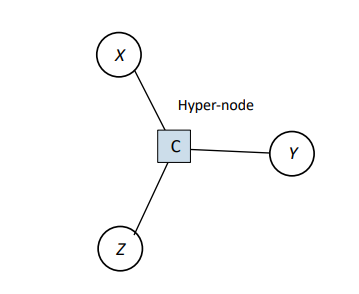
\includegraphics[scale=0.75]{5.png}
\end{center}
\subparagraph{Dual Graph transformation} Alternate way to convert a $n$-ary CSP to a binary one:
\begin{enumerate}
	\item Create a new graph in which there is one variable for each constraint in the original graph
	\item If two constraints share variables, they are connected by an arc corresponding to the constraint that the shared variables receive the same value
\end{enumerate}
Example: $Dom(x) = Dom(y) = Dom(z) = \{1,2,3\}$ with $C_1 = \{(x,y,z), x + y = z\} = \{(1,2,3), (2,1,3), (1,1,2)\}$ and $C_2 = \{(x,y), x < y\} = \{(1,2), (1,3), (2,3)\}$.
This will become $Dom(C_1) = \{(1,2,3), (2,1,3), (1,1,2)\}, Dom(C_2)=\{(1,2), (1,3), (2,3)\}$ and $R_{x,y} =$ constraint that $x$ and $y$ will receive the same values
\begin{center}
	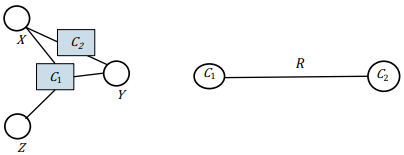
\includegraphics[scale=0.75]{6.png}
\end{center}
\paragraph{Related concepts} \begin{list}{}{}
	\item \textbf{Problem reduction techniques}: techniques for transforming CSP into an equivalent problem easier to solve or recognizable as insoluble
	\item \textbf{Enforcing local consistency}: the process of enforcing local consistency properties in a constraint graph causes inconsistent values to be eliminated. Different types of local consistency properties have been studied.
	\item \textbf{Constraint propagation/inference}: constraints are used to reduce the number of legal values for a variable, which in turn can reduce the legal value for another variable and so on\ldots
\end{list}
\subparagraph{Problem reduction} Reducing a problem means removing those constraints which appear in no solution tuples.\\
A CSP problem $P_1$ is reduced to $P_2$ when $P_1$ is equivalent to $P_2$, domains of variables in $P_2$ are subsets of those in $P_1$ and the constraints in $P_2$ are at least as restrictive as those in $P_1$.\\
These conditions guarantees that a solution in $P_2$ is also a solution in $P_1$.\\
\textbf{Problem reduction strategies} are of two types: removing redundant values from the domains of the variables or tightening the constraints so that fewer compound labels satisfy them (examples: if $x < y$ and $D_x = \{3,4,5\}, D_y = \{1, 2,4\}$ then those can be reduced to $D_x=\{3\}, D_y=\{4\}$.\\
Constraints are sets, this means removing redundant compound labels from the set. If the domain of any variable or any constraint is reduced to an empty set, then the problem is \textbf{unsolvable}.\\
Problem reduction is also called consistency checking or maintenance, since it relies on establishing local consistency properties.\\\\
\textbf{Local consistency properties}: node consistency, arc consistency, path consistency, k-consistency, forward checking.\\
All these operations do not change the set of solutions, do not necessarily solve a problem but, used with search, will make the search more efficient by pruning the search tree.
\begin{list}{}{} 
	\item \textbf{Node/Domain consistency}: a node is consistent if all the values in its domain satisfy unary constraints on the associated variable. A constraint network is node-consistent if all the nodes are consistent.\\
	Given a unary constraint on $x_i$, $C_i = \langle(x_i), R_i\rangle$ then node consistency $D_i \subseteq R_i$ and can be enforced by reducing the domains of the variables $D_i \leftarrow D_i \cap R_i$ (this is the NC-1 algorithm, $O(d\cdot n)$)
	\item \textbf{Arc consistency}: a variable is arc-consistent if every value in its domain satisfies the binary constraints of this variable with other variable. $x_i$ is arc-consistent with respect to $x_j$ if for every value in its domain $D_i$ there is some value in the domain $D_j$ that satisfies the binary constraint on the arc $(x_i, x_j)$\\
	Example, $X = \{x, y\}$, $D_x = D_y = \{0,1,2,3,4,5,6,7,8,9\}$ and constraint $\langle(x,y), x=y^2\rangle$. Considering arc $x \rightarrow y$, it can be made consistent by reducing $D_x$ to $\{0,1,4,9\}$. Considering $y \rightarrow x$, can be made consistent by reducing $D_y$ to $\{0,1,2,3\}$, making the entire edge consistent.
\end{list}
\paragraph{Arc Consistency Algorithm (AC-3)} It maintains a queue of arcs to consider, initially all the arcs in CSP. An edge produces two arcs. AC-3 pops off an arc $(x_i, x_j)$ from the queue and makes $x_i$ arc-consistent with respect to $x_j$: \begin{list}{}{}
	\item If this step leaves $D_i$ unchanged, the algorithm just moves on to the next arc
	\item If $D_i$ is made smaller, then we need to add to the queue all arcs $(x_k, x_j)$ where $x_k$ is a neighbor of $x_i \neq x_j$
	\item If $D_i$ becomes empty, then we conclude that the CSP has no solution
\end{list}
When there are no more arcs to consider, we have finished: we are left with a CSP equivalent to the original but smaller.\\
With a CSP of $n$ variables, each with domain size at most $d$ and $c$ binary constraints (arcs):
\begin{list}{}{}
	\item Checking consistency of an arc can be done in $O(d^2)$ time
	\item Each arc $(x_i, x_j)$ can be inserted in the queue only $d$ times (because $x_i$ has at most $d$ values to delete)
	\item We have $c$ arcs to consider, so complexity is $O(c\cdot d^3)$, polynomial time
\end{list}
The AC-4 algorithm is an improved version of AC-3, based on the notion of support that doesn't need to consider all the incoming arcs. More information is kept, but complexity is $O(c\cdot d^2)$.
\subparagraph{Example} $A, B, C \in \{1,2,3,4\}, A < B, A > C$\\
\begin{center}
\begin{tabular}{c c c}
	Queue & Arc & Arc domain\\
	\hline
	$\{(A,B), (B, A), (A, C), (C, A)\}$ & & \\
	$\{(B, A), (A, C), (C, A)\}$ & $(A,B)$ & $A \in \{1,2,3,\not 4\}$ \\
	$\{(A,C), (C, A)\}$ & $(B, A)$ & $B \in \{\not 1, 2, 3, 4\}$\\
	$\{(C, A)\}$ & $(A, C)$ & $A \in \{\not 1, 2, 3\}$\\
	$\{(B,A), (C, A)\}$ & & \\
	$\{(C, A)\}$ & $(B, A)$ & $B \in \{\not 2, 3, 4\}$\\
	$\{\}$ & $(C, A)$ & $C \in \{1, 2, \not 3,\not 4\}$\\
\end{tabular}
\end{center}
At the end $A\in\{2,3\}, B\in\{3,4\}, C\in\{1,2\}$
\paragraph{Directional Arc Consistency} DAC is defined with reference to a total ordering of the variables. A CSP is DAC under an ordering of the variables if and only if for every label $\langle x, a\rangle$ which satisfies the constraints on $x$ there exists a compatible label $\langle y,b\rangle$ for every label $y$ which is after $xc$ according to the ordering.\\
In the algorithm for establishing DAC (DAC-1) each arc is examined exactly once, by proceeding from last to the first in the ordiering, so the complexity is $O(c\cdot d^2)$. AC cannot always be achieved by running DAC-1 in both directions.
\paragraph{Generalized Arc Consistency} GAC, extension of AC-3 to handle $n$-ary constraints rather than just binary. A variable $x_i$ is GAC with respet to a $n$-ary constraint if for every value $v$ in the domain of $x_i$ there exists a tuple of values that is a member of the constraint and has its $x_i$ component equal to $v$.\\
For example, if $X, y, Z \in \{0,1,2,3\}$ and $X < Y < Z$, to make $C$ consistent we would have to eliminate $2, 3$ from the domain of $X$ because the constraint cannot be satisfied with $X=2$ or $X=3$.
\paragraph{Path Consistency} Arc consistency tightens down the domains using the arcs (binary constraints). Path consistency is a stronger notion: tightens the binary constraints by using implicit constraints that are inferred by looking at the triples of variables. A path of length 2 between variables $x_i, x_j$ is path-consistent with respect to a third intermediate variable $x_m$ if for every consistent assignment $\{x_i = a, x_j = b\}$ there is an assignment to $x_m$ that satisfies the constraints on $(x_i, x_m)$ and $(x_m, x_j)$. In relational algebra $R_{i,j}\subseteq\pi_{i,j}(R_{i,m}\bowtie D_m\bowtie R_{m,j})$\\
To achieve path consistency, $R_{i,j}\leftarrow R_{i,j}\cap\pi_{i,j}(R_{i,m}\bowtie D_m\bowtie R_{m,j})$ (algorithm name: PC-2). If all path of length 2 are made consistent, then all paths of any length are consistent.\\
Called path consistency because you can think of it as a path from $x_i$ to $x_j$ with $x_m$ in the middle.
\paragraph{Combining search and problem reduction} Problem reduction techniques are used in combination with search. The more effort one spends on problem reduction, the less effort one needs in searching.
\begin{center}
	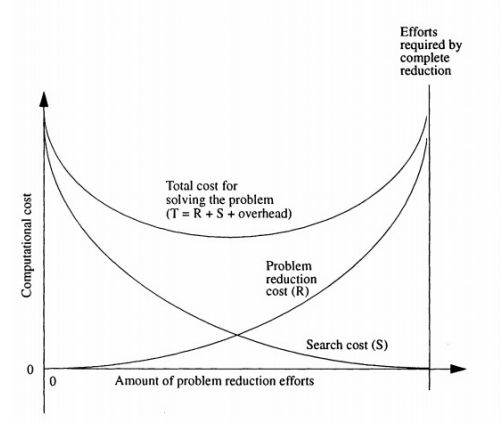
\includegraphics[scale=0.75]{7.png}
\end{center}
Most problems cannot be resolved by reduction alone, we must search for solutions and combine problem reduction with search. In this context we talk about \textbf{constraint propagation} or \textbf{inference}. A classical incremental formulation of CSP as a search problem is:
\begin{list}{}{}
	\item States are partial assignments
	\item Initial state: empty assignment
	\item Goal state: complete assignment that satisfy all constraints
	\item Actions: assign to a specific unassigned variable $x_i$ a value $\in D_i$
\end{list}
Branching factor: $d$, with $d$ maximum cardinality of the domains. Number of leaves: $d^n$, with $n$ number of variables. $n$ finite $\Rightarrow$ space graph finite.
\paragraph{CSP as search: simplifications} We can exploit \textbf{commutativity}. A problem is commutative if the order of application of any given set of action has no effect on the outcome. In this case, the order of the variable assignments does not change the result.\\
We can consider a single variable for assignment at each step, so the branching factor is $d$ and the number of leaves id $d^n$. We can also exploit depth limited search: \textbf{backtracking search} with depth limit $n$.\\
Search strategies:
\begin{list}{}{}
	\item \textbf{Generate and Test}: generate a full solution and test it, not the best
	\item \textbf{Anticipated Control}: after each assignment we check the constraint, if some is violated we backtrack to previous choices (undoing the assignment)
\end{list}
\paragraph{Backtracking search algorithm}  %TODO code
\paragraph{Heuristics and search strategies}
\begin{list}{}{}
	\item \texttt{SELECT-UNASSIGNED-VARIABLE}: which variable should be assigned next?
	\item \texttt{ORDER-DOMAIN-VALUES}: in which order should the values be tried?
	\item \texttt{INFERENCE}: what inference should be performed at each step?\\
	Techniques for \textbf{constraint propagation} (local consistency enforcement) can be used
	\item \texttt{BACKTRACKING}: where to back up to? When the search ends up in an assignment that violates a constraint, can the search avoid repeating this failure? Forms of \textbf{intelligent backtracking}
\end{list}
\subparagraph{Choosing the next variable}\begin{list}{}{}
	\item \textbf{MRV} (minimnum remaining values): variable with fewest "legal" remaining values
	\item \textbf{Degree heuristic}: variable involved in the largest number of constraints
\end{list}
\subparagraph{Choosing value} \begin{list}{}{}
	\item \textbf{Least constaint variable}: prefer the variable rules out the fewest choices
\end{list}
Note that in choosing the variable, a fail-first strategy helps in reducing the amount of search by pruning large parts of the tree earlier. In the choice of value, a fail-last approach works best in CSP where the goal is to find \textit{any} solution. This is not effective if we are looking for all solutions or no solution exists.
\subparagraph{Interleaving search and inference} One of the simplest form of inference propagation is \textbf{forward checking}: efficient constraint propagation, weaker than other forms. Whenever $X$ is assigned, FC process establishes arc consistency of $X$ for the arcs connecting neighbor nodes. For each unassigned $Y$ connected to $X$, delete from $Y$'s domain any value inconsistent with the value assigned to $X$.
\subparagraph{Constraint learning} When the search is at a contradiction, we know that some subset of the conflict set is responsible. Constraint learning is the idea of finding a minimum set of variables from the conflict set that causes the problem: the no-good set. We record the no-good set either by adding a new constraint to CSP or by keeping a separate cache of no-goods. This way we do not repeat the no-good state.

\paragraph{Local search} Requires a complete state formulation, keep in memory only current state to improve it iteratively and does not guarantee to find a solution even if it exists (\textbf{not complete}).\\
Used when space too large for systematic search and we need to be very efficient. Also when we need to provide a solution but it's not important to produce solution path. Also when we know in advance that a solution exists.
\subparagraph{Local search methods for CSP} Complete state formulation: we start with a complete random assignment, and we try to fix it until all the constraints are satisfied.\\
Local methods are very efficient for large scale problems where the solutions are densely distributed in the space. A basic algorithm is:
\begin{verbatim}
function Local_search(V, Dom, C) returns a complete & consistent assignment
Inputs: V: a set of variables
Dom: a function such that Dom(x) is the domain of variable x
C: set of constraints to be satisfied
Local: A (complete assignement) an array of values indexed by variables in V

repeat until termination
for each variable x in V do # random initialization or random restart
A[x] := a random value in Dom(x)
while not stop_walk( ) & A is not a satisfying assignment do # local search
Select a variable y and a value w in Dom(y), w != A[y] # a successors
A[y] := w # change a variable
if A is a satisfying assignment then return A # solution found
\end{verbatim}
this can be specialized, two extreme versions are: \textbf{random sampling} (no walking done to improve solution, so \texttt{stop\_walk} always \texttt{true}, just generating random assignments and testing them) or \textbf{random walk} (no restarting is done, so \texttt{stop\_walk} always \texttt{false})
\subparagraph{Heuristic Local Search} Inject heuristics in the selection of the variable and the value by the means of an evaluation function (in CSP, $f$ = \# violated constraints or conflicts, perhaps with weights).\\
\textbf{Iterative best improvement}: choose the successor that most improves the current state according to an evaluation function $f$. Moves to best successor even if worse than current state, may be stuck in loops, not complete.
\subparagraph{Stochastic Local Search} Adds randomness, escapes local minima:\begin{list}{}{}
	\item \textbf{Random restart} is a global random move: the search starts from a completely different part of the search state
	\item \textbf{Random walk} is a local random move: random steps are taken interleaved with the optimizing steps
\end{list}
There are possible variants \begin{list}{}{}
	\item Most improving step: selects a variable-value pair that makes the best improvement. Needs to evaluate all of them, needing strategies for efficient computation
	\item Two stage choice: select the variable that participates in most conflicts, then the value that minimizes conflicts (or a random value)
	\item Any conflict: choose a conflicting variable at random, select the value that minimizes conflicts (or a random value)
\end{list}
\paragraph{CSP: Min-Conflict Heuristic} All the local search techniques are candidate for CSP, some have proved especially effective. Min-conflict heuristics is widely used and also quite simple:
\begin{list}{}{}
	\item select a variable at random among the conflicting variables
	\item select the value that results in the \textbf{minimum number of conflicts} with other variables
\end{list}
%TODO algorithm
\subparagraph{Improvements} Usually many plateaux, possible improvements:
\begin{list}{}{}
	\item \textbf{Tabu Search}: local search has no memory, the idea is keeping a small list of the last $t$ steps and forbidding the algorithm to change the value of a variable whose value was changed recently. This is meant to prevent cycling among assignments, and $t$ is called \textbf{tenure}
	\item \textbf{Constraint Weighting}: concentrates the search on important constraints. We assign a numeric weight to each constraint, initially 1. The weight is incremented each time the constraint is violated: goal is choose the variable and value which minimizes the weights of the violated constraints.
\end{list}
\subparagraph{Alternatives}\begin{list}{}{}
	\item \textbf{Simulated Annealing}: allows downhill moves at the beginning of the algorithm and slowly \textit{freezes} this possibility
	\item \textbf{Population based methods}
	\begin{list}{}{}
		\item \textbf{Local Beam Search}: proceed with the $k$ best successors according to the evaluation function
		\item \textbf{Stochastic Local Beam Search}: selects $k$ of the individuals at random with a probability that depends on the evaluation function
		\item \textbf{Genetic Algorithms}\ldots
	\end{list}
\end{list}
\subparagraph{Online search} Another advantage of local search methods is that they can be used in an online setting when the problem changes dynamically.
\subparagraph{Evaluating randomized algorithms} Randomized algorithms are difficult to evaluate since they output a different result and a different execution time each time they run. We take the runtime distribution, which shows the number of runs in which the algorithm solved the problem within a given number of steps.\\
A randomized algorithm can be run multiple times with random restart, increasing the probability of success. An algorithm that succeeds with probability $p$ run $n$ times will found a solution with probability $1 - (1-p)^n$ with $(1-p)^n$ the probability of failing $n$ times.
%TODO CSP-4.pdf
\paragraph{Independent sub-problems: complexity}
\paragraph{The structure of problems: tree} In a tree-structured graph, two node are connected by only one path: we can choose any variable as root of the tree. Chosen a variable as root, the tree induces a topological sort on the variables: chieldren of a node are listed after their parent
\subparagraph{Directional arc consistency} %TODO def
\paragraph{Reducing graphs to trees} For example, assigning a value to the node we want to remove and removing inconsistent values for other variables, then solve with tree-csp-solver.\\
In general not easy.
\subparagraph{Cutset conditioning} Domain splitting strategy, trying with different assignments: choose subset S of CSP's variabile such that the constraint graph becomes a tree: S is cycle cutset. For each consistent assignmetn to variabiles in S: remove from the domains of remaining vars any vals that are inconsistent, if the remaining CSP has a solution, return it together with the current assignment of S.\\
Time $O(d^c(n-c)d^2)$ where $c$ is size of cycle cutset and $d$ size of the domain. We have to try each of the $d^c$ coimbinations of values for the cvaraibles in $S$ and for each combination we must solve a tree problem of size $(n-c)$
\paragraph{Tree decomposition} The approach consists in a tree decomposition of the contrasint graph into a set of connected sub-roboelkms. Each of them is solved intdepentendly\ldots\\ %TODO with image
\begin{list}{}{}
	\item every var in the original problem appears in at least one of the sub-problems
	\item if two var connectd by a constraint they must appear together at least in one of the sub problem along with the constraint
	\item if a variabile appears in two subproblems in the tree, it must appear in every subproblem along the path connecting those subproblems
\end{list}
1-2 ensure that all vars and constraints are represented. Condition 3 ensure that any given pvar must have same value in every subproblem.
\subparagraph{Solving a decomposed problem} %TODO
\paragraph{Simmetry} important factor for reducing complexity of CSP problems. Value simmetry: the values does not really matter: different colors, but there are 6 equivalent ways of satisfying the constraints. If $S$ is as solution to coloring $n$ var, there are $n!$ solutions.\\
\textbf{Simmetry breaking constraints}: we impost an arbitrary ordering constraints that requires the values to be in alphabetical order. Breaking value simmetry has proved to be important and effective on many problems.
\end{document}